\documentclass{article}
\usepackage[utf8]{inputenc}
\usepackage{amsmath,amsthm,amssymb}

\title{Solution Mannual for Supplyment Psets of MIT OCW 18.02SC Fall 2010}
\author{Lu YuXun}
\date{February 2017}

\usepackage{natbib}
\usepackage{graphicx}
\linespread{1.5}
\begin{document}

\maketitle

\section{Vectors and Matrices}
\subsection{A. Vectors}
\textbf{1A-12*} Label the four vertices of a parallelogram in counterclockwise order as OPQR. Prove that the line segment from O to the midpoint of PQ intersects the diagonal PR in a point X that is 1/3 of the way from P to R.
\begin{figure}[htp!]
    \centering
    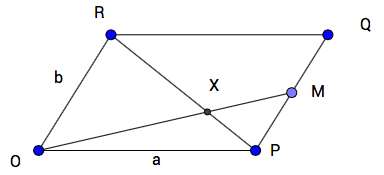
\includegraphics[width=50mm,scale=0.5]{Figure/1A-12.png}
    \caption{1A-12 Figure}
    \label{1A-12 Figure}
\end{figure}
\begin{proof}
Suppose $\overrightarrow{OP} = \mathbf{a}$ and $\overrightarrow{OR} = \mathbf{b}$.
\\ We have: $\overrightarrow{RP} = \mathbf{a} - \mathbf{b}$ (1), $\overrightarrow{OM} = \mathbf{a} + \frac{1}{2} \mathbf{b}$ (2), $\overrightarrow{OX} = \mathbf{b} + \overrightarrow{RX}$ (3).
\\Let $\overrightarrow{OX} = u(\mathbf{a} + \frac{1}{2}\mathbf{b})$, $\overrightarrow{RX} = (1 - v)(\mathbf{a} - \mathbf{b})$.
\\ From (3) we can derive:
\\ $\mathbf{b} + \overrightarrow{RX} = \overrightarrow{OX} = u\mathbf{a} + \frac{u}{2}\mathbf{b} = \mathbf{b} + (1-v)\mathbf{a} - (1-v)\mathbf{b}$
that is, 
\begin{equation}
    \begin{cases}
    u = 1 - v
    \\ v = \frac{u}{2}
    \end{cases}
\end{equation}
Solve equations in (1), we have $u = \frac{2}{3}, v = \frac{1}{3}$. So $\overrightarrow{OX} = \frac{2}{3} \overrightarrow{OM}$ and $\overrightarrow{RX} = \frac{2}{3} \overrightarrow{RP}$, i.e. the intersection point X of RP and OM is 1/3 of the way from P to R.
\end{proof}
\textbf{1A-13*} a) Take a triangle $PQR$ in the plane; prove that as vectors $PQ+QR+RP = 0$.
\\ b) Continuing part a), let \textbf{A} be a vector the same length as $PQ$, but perpendicular to it, and pointing outside the triangle. Using similar vectors \textbf{B} and \textbf{C} for the other two sides, prove that \textbf{A} + \textbf{B} + \textbf{C} = \textbf{0}. (This only takes one sentence, and no computation.)
\begin{proof}
a) $\because \overrightarrow{PQ} + \overrightarrow{QR} = \overrightarrow{PR}, \overrightarrow{PR} = -\overrightarrow{RP}$
\\ $\therefore \overrightarrow{PQ} + \overrightarrow{QR} + \overrightarrow{RP} = \mathbf{0}$
\\ b) Because the triangle constructed by the segment lines of \textbf{A} and \textbf{B} and \textbf{C} is the triangle $\bigtriangleup PQR$ rotated 90 degrees, since we have proved that the three vectors consisting of the three sides of $\bigtriangleup PQR$ add to \textbf{0}, \textbf{A} + \textbf{B} + \textbf{C} = \textbf{0}.
\end{proof}
\textbf{1A-14*} Generalize parts a) and b) of the previous exercise to a closed polygon in the plane which doesn't cross itself (i.e., one whose interior is a single region); label its vertices $P_1, P_2,...,P_n$ as you walk around it.
\begin{proof}
We are going to use strong induction. 
\\Suppose $P(n)$: for a closed polygon with $n$ sides, $\overrightarrow{P_1P_2} + \overrightarrow{P_2P_3} + \overrightarrow{P_3P_4} + ... + \overrightarrow{P_{n-1}P_n} + \overrightarrow{P_nP_1} = \mathbf{0}$, $n \in \mathbb{N}^+ \wedge n \geq 3$.
\\ \textit{Base Case} P(3) is true, since we have proved it in \textbf{1A-13*} (a) part.
\\ \textit{Inductive Step} Suppose $P(1), P(2), ..., P(n)$ is true. For $P(n+1)$, we could add up arbitrary two adjacent vectors to eliminate one side, i.e. let $\overrightarrow{P_iP_{i+2}} = \overrightarrow{P_iP_{i+1}} + \overrightarrow{P_{i+1}P_{i+2}}$ where $ 3 \leq i \leq n+1 \wedge i \in \mathbb{N}^+$. So $P(n+1)$ decays to $P(n)$ and by our inductive assumption, $P(n)$ is true. Thus, $P(n+1)$ is true, i.e. $P(n) \implies P(n+1)$. So $P(n)$ is true for all positive nature number $n \geq 3$
\end{proof}
\end{document}